\renewcommand{\thefigure}{A\arabic{figure}}
\setcounter{figure}{0}
\renewcommand{\thetable}{A.\arabic{table}}
\setcounter{table}{0}
\renewcommand{\thesection}{A.\arabic{section}}
\setcounter{section}{0}

\section*{Appendix}

\subsection*{PTS Civil War Robustness Check}

\begin{figure}
    \centering
    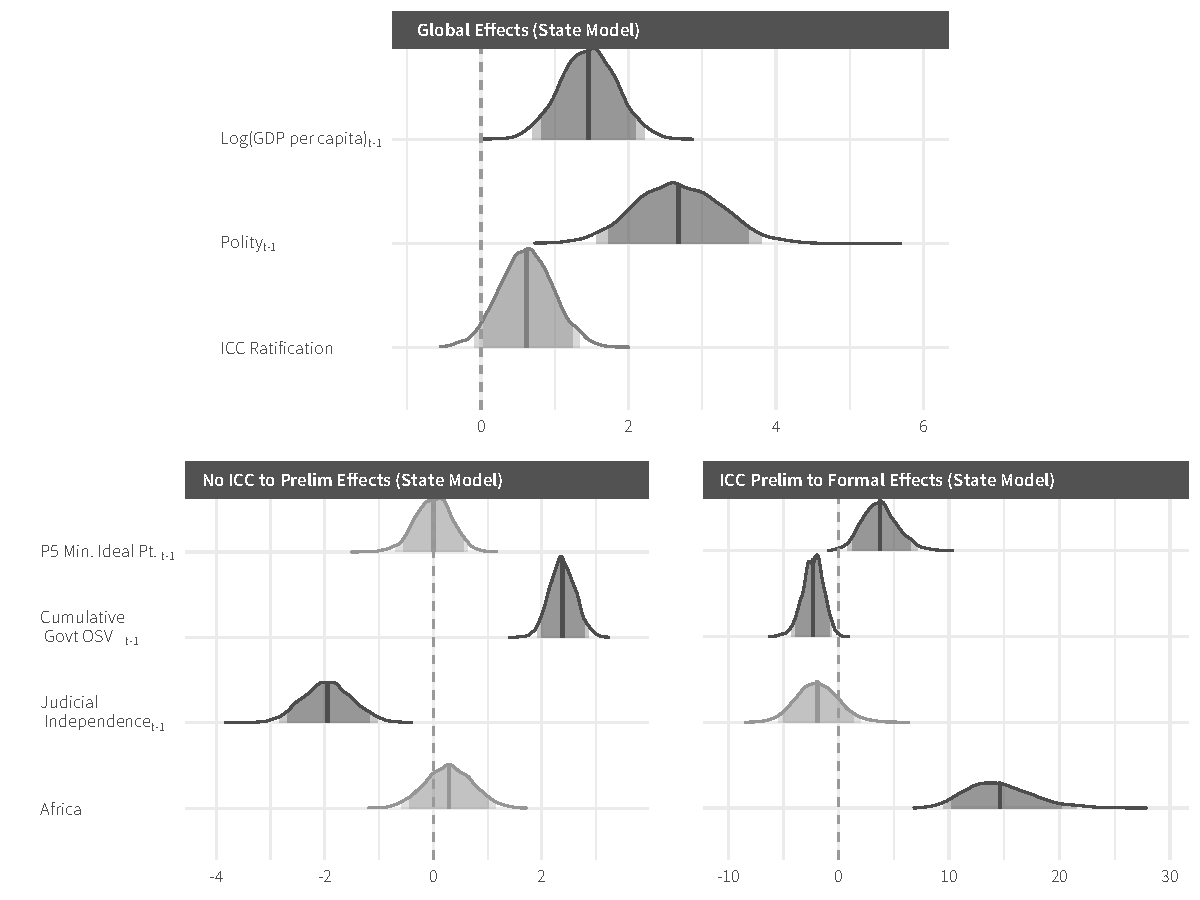
\includegraphics[width=1\textwidth]{stateCoefSumm_ptsCivilWarOnly.pdf}
    \caption{Parameter estimates from State-Focused ICC Transition model visualized through posterior distributions with median values designated by vertical line, lightly shaded portion indicating the 95\% credible interval, and darker shaded portion the 90\% credible interval.}
    \label{fig:stateModel}
\end{figure}

\begin{figure}
    \centering
    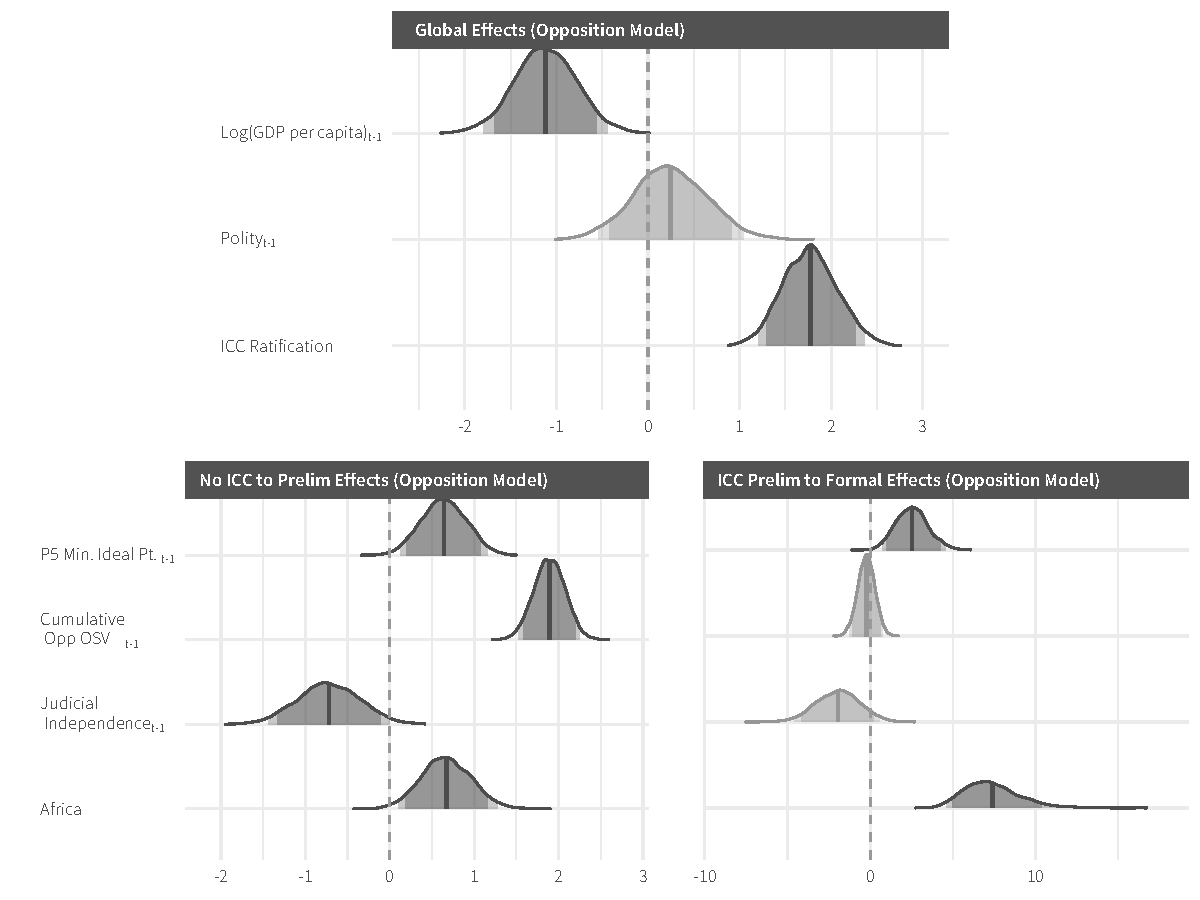
\includegraphics[width=1\textwidth]{rebelCoefSumm_ptsCivilWarOnly.pdf}
    \caption{Parameter estimates from Opposition-Focused ICC Transition model visualized through posterior distributions with median values designated by vertical line, lightly shaded portion indicating the 95\% credible interval, and darker shaded portion the 90\% credible interval.}
    \label{fig:rebelModel}
\end{figure}

\subsection*{Comparison with ordinal logit}

Marginal effects different

Performance comparison

\subsection*{MCMC sampler}


\subsection*{Stan Code}



% latex table generated in R 3.5.0 by xtable 1.8-2 package
% Fri Feb  1 20:29:20 2019
% \begin{table}[ht]
% \centering
% \begingroup\footnotesize
% \begin{tabular}{lcc}
%  Variable & state & rebel \\
%   \hline
% \hline
% icc rat & $1.23^{\ast\ast}$ & $2.02^{\ast\ast}$ \\
%   & (0.27) & (0.26) \\
%   lag1 civilwar & $2.72^{\ast\ast}$ & $2.41^{\ast\ast}$ \\
%   & (0.27) & (0.26) \\
%   lag1 polity2 & $0.13^{\ast\ast}$ & 0.01 \\
%   & (0.03) & (0.03) \\
%   lag1 gdpCapLog & $0.43^{\ast\ast}$ & $-0.25^{\ast\ast}$ \\
%   & (0.09) & (0.11) \\
%   africa[1] & 0.24 & $0.81^{\ast\ast}$ \\
%   & (0.29) & (0.25) \\
%   africa[2] & $10.74^{\ast\ast}$ & $6.42^{\ast\ast}$ \\
%   & (2) & (1.46) \\
%   lag1 osv rebel cumul[1] &  & $0.15^{\ast\ast}$ \\
%   &  & (0.04) \\
%   lag1 osv rebel cumul[2] &  & $-0.21^{\ast\ast}$ \\
%   &  & (0.09) \\
%   lag1 osv state cumul[1] & $0.2^{\ast\ast}$ &  \\
%   & (0.04) &  \\
%   lag1 osv state cumul[2] & $-0.6^{\ast\ast}$ &  \\
%   & (0.16) &  \\
%   lag1 p5 absidealdiffMin[1] & -0.58 & 0.53 \\
%   & (0.47) & (0.49) \\
%   lag1 p5 absidealdiffMin[2] & $6.46^{\ast\ast}$ & $4.1^{\ast\ast}$ \\
%   & (2.59) & (1.87) \\
%   lag1 v2juncind[1] & $-0.81^{\ast\ast}$ & $-0.43^{\ast\ast}$ \\
%   & (0.12) & (0.13) \\
%   lag1 v2juncind[2] & -0.35 & $-0.98^{\ast\ast}$ \\
%   & (0.58) & (0.48) \\
%   \hline
% \hline
% \end{tabular}
% \endgroup
% \caption{$^{**}$ and $^{*}$ indicate significance at $p< 0.05 $ and $p< 0.10 $, respectively.}
% \end{table}
